\documentclass[12pt]{article}
\usepackage[a4paper]{geometry}
\usepackage[myheadings]{fullpage}
\usepackage{fancyhdr}
\usepackage[table,xcdraw]{xcolor}
\usepackage{array,multirow,makecell}
\usepackage{lastpage}
\usepackage{graphicx, wrapfig, subcaption, setspace, booktabs}
\usepackage[T1]{fontenc}
\usepackage[font=small, labelfont=bf]{caption}
\usepackage{fourier}
\usepackage[protrusion=true, expansion=true]{microtype}
\usepackage[english]{babel}
\usepackage{sectsty}
\usepackage{url}
\usepackage{enumerate}
\usepackage{enumitem}
\usepackage{mdframed}
\usepackage{soul}
\usepackage{amsmath}
\usepackage{amssymb}
\usepackage{alltt}
\usepackage{fullpage}
\usepackage[table,xcdraw]{xcolor}

\singlespacing
\setcounter{tocdepth}{5}
\setcounter{secnumdepth}{5}

%-------------------------------------------------------------------------------
% HEADER & FOOTER
%-------------------------------------------------------------------------------
\pagestyle{fancy}
\fancyhf{}
\setlength\headheight{12pt}
\fancyhead[R]{Garza, Baker, and Sah \thepage}
\fancyhead[L]{Western Michigan University}
%-------------------------------------------------------------------------------
% TITLE PAGE
%-------------------------------------------------------------------------------
\begin{document}
\begin{titlepage}
    \newcommand{\HRule}{\rule{\linewidth}{0.5mm}} % Defines a new command for horizontal lines, change thickness here
    
    \center % Center everything on the page
    
    %----------------------------------------------------------------------------------------
    %	HEADER SECTION
    %----------------------------------------------------------------------------------------
    
    \textsc{\LARGE Western Michigan University}\\[0.5cm]
    \textsc{\Large Department of Electrical and Computer Engineering}\\[0.5cm] 
    \textsc{\large ECE-4820 Senior Design II}\\[0.5cm] 
    
    %----------------------------------------------------------------------------------------
    %	TITLE SECTION
    %----------------------------------------------------------------------------------------
    
    \HRule \\[0.4cm]
    { \huge \bfseries  Claims-Investigation Committee (CIC) Multi-Input Testing Device}\\[0.4cm]  
    \textsc{\Large Final Report (Outline/Draft)}\\[0.4cm] 
    \HRule \\[1.5cm]
    
    %----------------------------------------------------------------------------------------
    %	LOGO SECTION
    %----------------------------------------------------------------------------------------
    
    
\includegraphics[width=0.3\textwidth]{./../assets/WMU_Logo.png}\\[1cm]  
    %----------------------------------------------------------------------------------------
    %	DATE SECTION
    %----------------------------------------------------------------------------------------
    
    {\large \today}\\[1cm] 
    
    %----------------------------------------------------------------------------------------
    %	ADVISOR & SPONSOR SECTION
    %----------------------------------------------------------------------------------------
    
    \begin{minipage}{0.4\textwidth}
        \begin{flushleft} \large
            \emph{Faculty Advisor:}\\
            Dr. Janos Grantner\\ [.25cm]
        \emph{Team Members:}\\
        Dylan-Matthew Garza\\
        Daniel Baker\\
        Rohullah Sah
        \end{flushleft}
    \end{minipage}
    ~
    \begin{minipage}{0.4\textwidth}
        \begin{flushright} \large
            \emph{Sponsor:} \\
            ZF
            \\\emph{Contact:}\\
            Patrick McNally\\ 
            Patrick.McNally@zf.com
        \end{flushright}
    \end{minipage}\\[1cm]
    
    %----------------------------------------------------------------------------------------
    %	TEAM MEMBERS SECTION
    %----------------------------------------------------------------------------------------
    
    \begin{flushleft} \large
    \end{flushleft}
    
    \vfill 
    
\end{titlepage}

\tableofcontents
\newpage
%----------------------------------------------------------------------------------------
%	PAPER BEGINS WITH ABSTRACT
%----------------------------------------------------------------------------------------


\section{Abstract}
\begin{itemize}
  \item Summarize project need
    \begin{itemize}
      \item Ease of testing devices
      \item Technicians and engineers benefit 
    \end{itemize}
  \item Summarize project architecture 
    \begin{itemize}
      \item Custom PCB for device interfacing
      \item Using ARM Cortex-M4 for testing devices
      \item Embedded Linux running on ARM Cortex-A7
      \item Rust written Server to communicate to web-application and Cortex-M4 firmware
      \item Web application using WebAssembly for simple user interaction that provides a CSV
    \end{itemize}
  \item Summarize results 
    \begin{itemize}
      \item Measurements by X firmware had x\% accuracy 
      \item Total costs are X
    \end{itemize}
\end{itemize}

%----------------------------------------------------------------------------------------
%	OVERVIEW STARTING WITH INTRODUCTION
%----------------------------------------------------------------------------------------
\section{Introduction}
Describe Purpose and Scope of project

\begin{itemize}
  \item Project aims to simplify testing proceedures at ZF
  \item Utilize industry technology such as ARM processors and microcontrollers
    as well as Yocto Project for embedded Linux
  \item Use emerging technologies to solve real world problems (Rust programming 
    language and web assembly)
  \item Goal to have a functioning project.
\end{itemize}


%----------------------------------------------------------------------------------------
%	DISCUSSION PORTION
%----------------------------------------------------------------------------------------
\section{Discussion}
%----------------------------------------------------------------------------------------
%	Overview of Project
%----------------------------------------------------------------------------------------
\subsection{Background}


\subsection{Need Statement}
\begin{itemize}
  \item Describe current Device testing situation at ZF
  \item explain why it is suboptimal and current difficulties
  \item Explain who is affected (the engineers and technicians times')
\end{itemize}

\subsection{High-Level System Design}

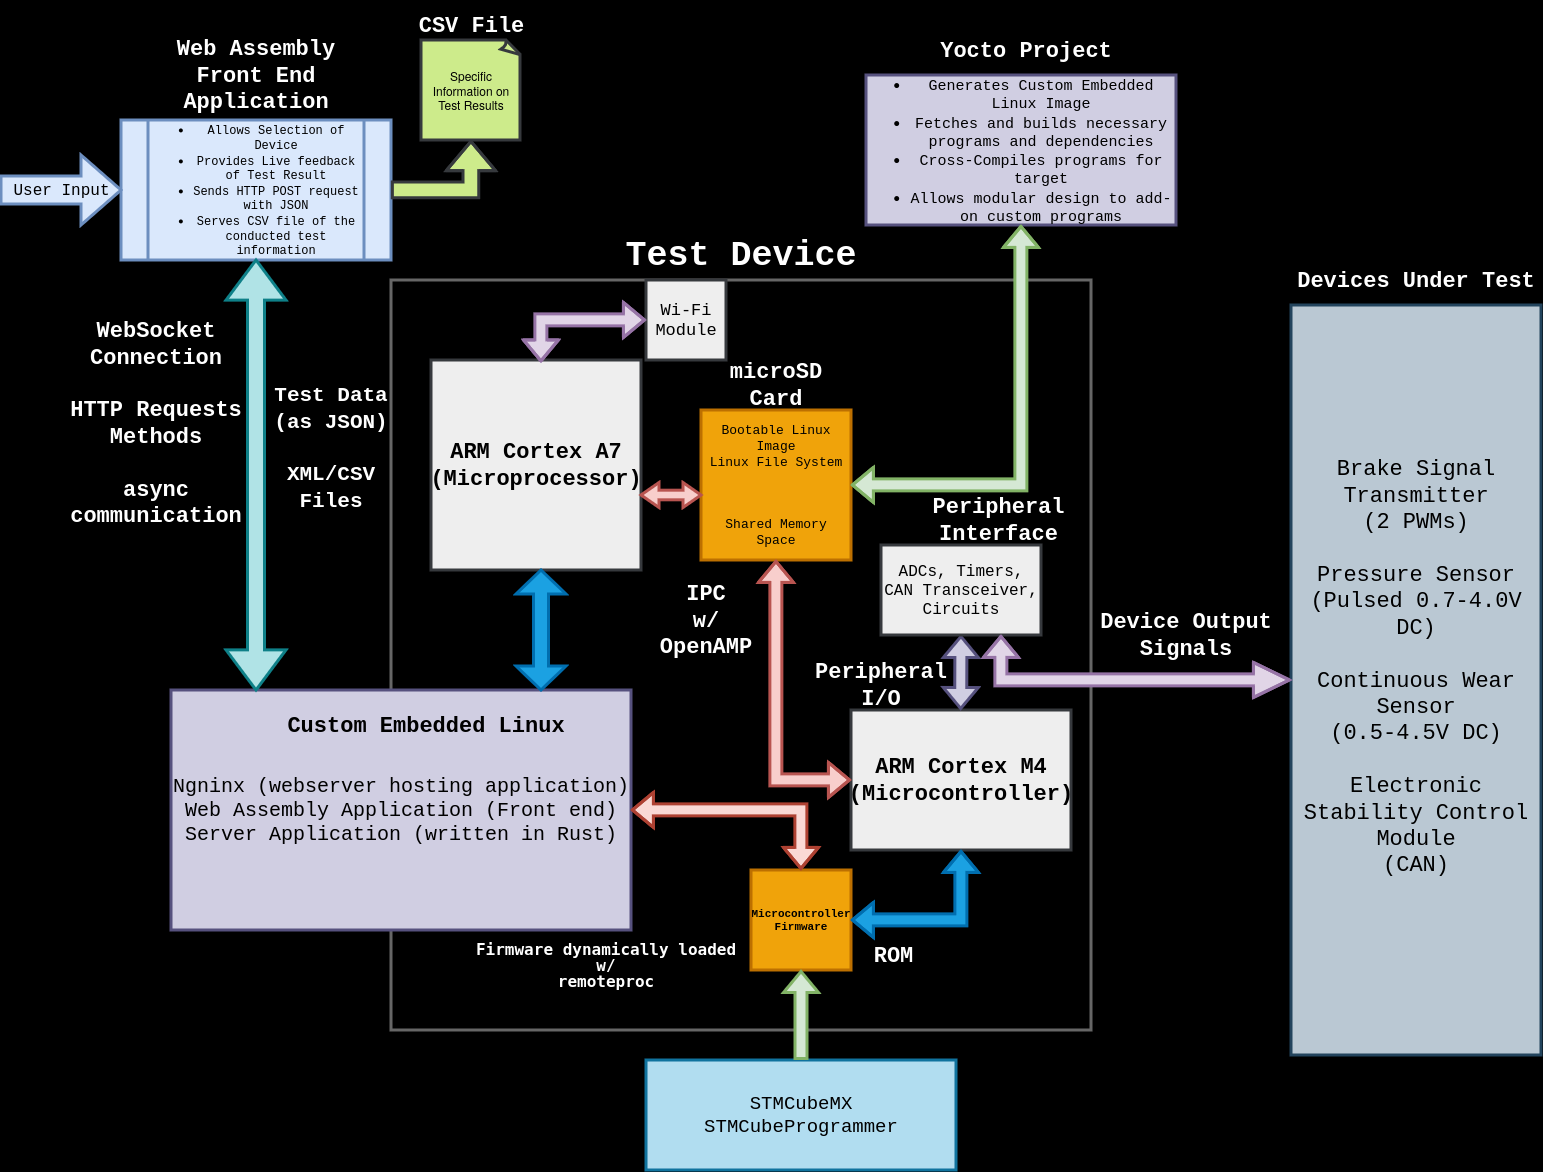
\includegraphics[width=\textwidth]{../assets/block_diagram.png}

\subsection{Specifications}
\begin{itemize}
  \item list PCB circuit specifics here as well as DUT specifications
  \item Heterogenous architecture with Cortex-A7 and Cortex-M4 processors
  \item Embedded Linux built with Yocto Project build system
  \item Custom Server API written in Rust
  \item Web Assembly application to interact with Server and microcontroller
\end{itemize}

\subsection{Deliverables}
\begin{itemize}
  \item Custom PCB schematic diagram with layout
  \item Verification of M4 firmware measuring correct values
  \item Project Gantt Chart estimated actual 
\end{itemize}


%----------------------------------------------------------------------------------------
%	Design and Implementation
% 
% * Hardware (Circuit/PCB) and device interfacing and power management
% * Enclosure Design
% * ARM Cortex-M4 Firmware
% * Embedded Linux with Yocto Project
% * Web Assembly application
% * Webserver
% * Inter-Processor Communication (IPC)
%----------------------------------------------------------------------------------------
\section{Design and Implementation}
\subsubsection{Custom Printed Circuit Board for Device interfacing and Power Management}

\subsection{Arm Cortex-M4 firmware for device Testing}

\subsection{Embedded Linux with Yocto Project}

\subsection{Custom API Web Server in Rust}

\subsection{Web Assembly Application using the Yew framework}


%----------------------------------------------------------------------------------------
%	Design Considerations 
%----------------------------------------------------------------------------------------
\subsection{Design Considerations}

\subsubsection{Public Health}

\subsubsection{Safety and Welfare}

\subsubsection{Global Impact}

\subsubsection{Cultural Impact}

\subsubsection{Social Impact}

\subsubsection{Environmental/Sustainability}

\subsubsection{Economic}


%----------------------------------------------------------------------------------------
%	Design Impacts
%----------------------------------------------------------------------------------------
\subsection{Design Impacts}

\subsubsection{Global}

\subsubsection{Economic}

\subsubsection{Environmental}

\subsubsection{Societal}


%----------------------------------------------------------------------------------------
%	Performance and Testing Analysis
%----------------------------------------------------------------------------------------
\subsection{Performance and Testing Analysis}


%----------------------------------------------------------------------------------------
%	Conclusion
%----------------------------------------------------------------------------------------
\section{Conclusion}


\end{document}
